\date{}
\title{}
\date{}
\usepackage{pgfplots}
\pgfplotsset{compat=1.16}
\begin{document}
\begin{frame}
    \titlepage
\end{frame}

\begin{frame}
\frametitle{last time}
    \begin{itemize}
    \item sawtooth pattern with loss-based congestion control
    \item congestion control and queues
        \begin{itemize}
        \item impracticality of running network at 100\%
        \item loss-based congestion control tends to fill buffers
        \end{itemize}
    \item self-clocking idea
        \begin{itemize}
        \item duplicate acks = extra packets in flight
        \end{itemize}
    \item sending new data during recovery
        \begin{itemize}
        \item estimating packets in flight v cwnd
        \end{itemize}
    \item TCP-fairness
    \end{itemize}
\end{frame}

\section{TCP variants}
\begin{frame}{``traditional'' TCP variant names}
\begin{itemize}
\item everything we've talked about as standard = NewReno
\vspace{.5cm}
\item Tahoe --- slow start + redo slow start on any loss + fast retransmit
\item Reno --- Tahoe + halve window size on dup ACKs
\item NewReno --- Reno + fast recovery (send extra during fast retransmit)
\item SACK --- NewReno + use selective acknowledgments
\end{itemize}
\end{frame}

\begin{frame}{more recent TCP variants}
\begin{itemize}
\item BIC, CUBIC --- loss-based schemes that vary increase/decrease algorithm
\item Vegas, BBR, FAST, Compound, Westwood --- schemes that use latency/bandwidth to detect congestion
    \begin{itemize}
    \item (later topic)
    \end{itemize}
\item (and there are many, many more)
\end{itemize}
\end{frame}




\subsection{CUBIC}
\begin{frame}
\frametitle{CUBIC: default congestion control today}
    \begin{itemize}
    \item default in Linux (since 2006), OS X (since 2014), Windows (since 2019)
        \begin{itemize}
        \item sysadmin has other options they can configure
        \item can be changed on connection-by-connection basis
        \end{itemize}
    \item includes improvements to recovery we'll talk about later
    \item but mostn notably has non-additive increase
    \end{itemize}
\end{frame}

\begin{frame}
    \frametitle{increase intuition}
    \begin{itemize}
        \item `standard' TCP basically has two increase algorithms:
        \item slow start --- quickly explore window sizes
        \item congestion avoidance --- slowly probe for maximum
        \vspace{.5cm}
        \item abrupt transition between these is suspect
            \begin{itemize}
            \item should have gradual exploration $\rightarrow$ fine-tuning switch
            \end{itemize}
        \item heuristic for when to use slow start-style is suspect
            \begin{itemize}
            \item half way from last loss $\approx$ guess?
            \end{itemize}
    \end{itemize}
\end{frame}

\begin{frame}
    \frametitle{CUBIC increase algorithm}
    \begin{itemize}
    \item big idea: faster increase when further away from window size of last loss
        \begin{itemize}
        \item cubic function with saddle point at that window size
        \item function parameterized by time since loss
        \end{itemize}
    \item intuition for `steady state':
        \begin{itemize}
        \item guess correct window size is close to last loss
        \item quickly get to around that window size
        \item search slowly/precisely around that size to fine tune size
        \end{itemize}
    \item intuition for non-steady state:
        \begin{itemize}
        \item try to quickly probe for roughly how small/big it is
        \item worry about getting more precise size on later `pass'
        \end{itemize}
    \end{itemize}
\end{frame}


\begin{frame}{}
\begin{tikzpicture}
\node (pic) {
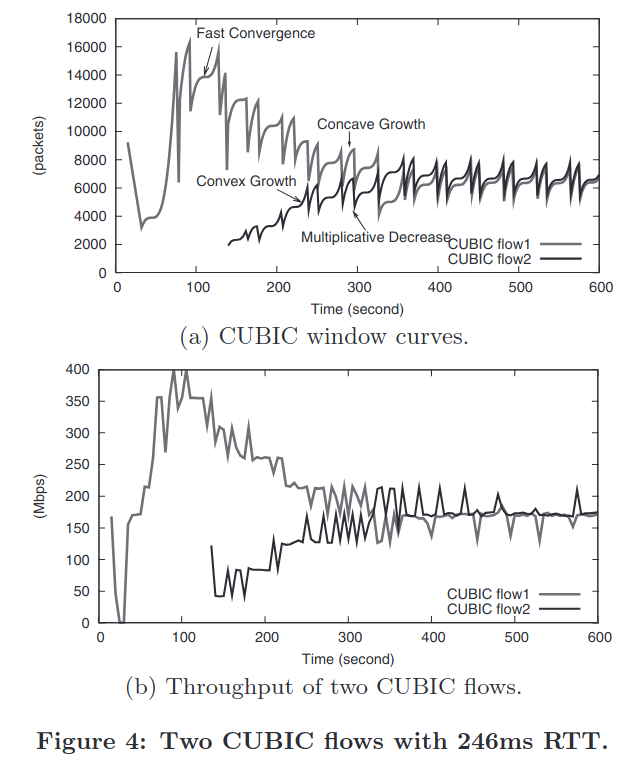
\includegraphics[height=\textheight]{../congest/cubic-fig4}
};
\node[anchor=north west,font=\tiny] at (pic.north east) {
from Ha, Rhee, and Xu, ``CUBIC: A New TCP-Friendly High-Speed TCP Variant''
};
\end{tikzpicture}
\end{frame}

\begin{frame}
    \frametitle{other CUBIC changes}
    \begin{itemize}
        \item different multiplicative decrease factor (divide by 1.4)
    \end{itemize}
\end{frame}


\section{other congestion signals}

\begin{frame}{other congestion signals}
\begin{itemize}
\item so far: detecting congestion via drops
    \begin{itemize}
    \item need data to go missing
    \item transmitting redundant data
    \item filling up buffers causing high latency
    \end{itemize}
\vspace{.5cm}
\item some alternate ideas:
\item have switches/routers `mark' packets
\item latency from longer queues
\end{itemize}
\end{frame}


\subsection{explicit congestion notification}
\againframe<2>{otherSig}
\begin{frame}{ECN}
\begin{itemize}
\item explicit congestion notification
\vspace{.5cm}
\item when buffer `close' to full
\item switches/router set `ECN' bit in some packets
    \begin{itemize}
    \item field in IP header
    \end{itemize}
\item ECN bit echoed back in ACKs
\end{itemize}
\end{frame}

\begin{frame}{ECN timeline}
\begin{tikzpicture}
\tikzset{
    box/.style={thick},
    message/.style={draw,thick,-Latex},
    failure/.style={draw,ultra thick,red,cross out,minimum width=1cm,minimum height=1cm},
    every node/.style={inner sep=0.1mm},
}
\begin{scope}[xshift=1cm,x=0.9cm]
\draw[box] (0, 0) rectangle ++(2, -6) 
    node[midway,align=center] {machine\\A};
\draw[box] (5, 0) rectangle ++(2, -6) 
    node[midway,align=center] {switch};
\draw[box] (13, 0) rectangle ++(2, -6) 
    node[midway,align=center] {machine\\B};
\draw[message] (2, -0.5) -- (13, -1.5) node[pos=0.25,above,sloped] {[no ECN]{0}: ``The ''}
    node[pos=0.75,above,sloped] {[no ECN]{0}: ``The ''};
\draw[message] (13, -1.75) -- (2, -2.75) node[pos=0.25,sloped,below] {got up to {0}};
\draw[message] (2, -1) -- (13, -2) node[pos=0.25, above, sloped] {[no ECN]{1}: ``meeting''}
    node[pos=0.75,above,sloped] {\myemph{[yes ECN]}{0}: ``The ''};
\draw[message] (13, -2.25) -- (2, -3.25) node[pos=0.25, sloped,below] {got up to {1} \myemph{WITH ECN mark}};

% in response to got 0
\draw[message] (2, -3) -- (13, -4) node[pos=0.5, above, sloped] {[no ECN] {2}: `` is at ''};
\draw[message] (13, -4.25) -- (2, -5.25) node[pos=0.25, sloped,below] {got up to {2}};
% in response to got 1
\draw[message] (2, -3.5) -- (13, -4.5) node[pos=0.5, above, sloped] {[no ECN] {3}: ``12pm.''};
\draw[message] (13, -4.75) -- (2, -5.75) node[pos=0.25, sloped,below] {got up to {3}};
\end{scope}
\end{tikzpicture}
\begin{itemize}
\item data sent has place for ECN bit to be placed
\item switch modifies ECN bit \myemph{if buffer close to full}
\item ACK indicates if ECN bit was set
\end{itemize}
\end{frame}



\subsection{watching latency, etc.}
\againframe<3>{otherSig}
\begin{frame}{very different congestion control}
    \begin{itemize}
    % FIXME: Fig 32 from TCPCC book
    \item fuller queues $\rightarrow$ higher latency
    \item fuller queues $\rightarrow$ throughput same as window increases
    \vspace{.5cm}
    \item<2-> strategy: monitor throughput/latency to detect full queues
        \begin{itemize}
        \item goal: fill link without making queue grow in size
        \item react before dropped packets happen
        \end{itemize}
    \end{itemize}
\end{frame}

\begin{frame}{`Vegas'-style congestion control}
    \begin{itemize}
    \item record ``base'' round-trip time
        \begin{itemize}
        \item connection start or lowest observed
        \end{itemize}
    \item ``ideal'' throughput should be one window / base round trip time
        \begin{itemize}
        \item (Vegas paper calls this ``expected'' throughput)
        \item what would happen with no queuing delay
        \end{itemize}
    \vspace{.5cm}
    \item goal: control what ``ideal'' - actual throughput is
        \begin{itemize}
        \item if 0, queues are probably empty, can increase window
        \item if large, queues are too big, decrease window
        \end{itemize}
    \end{itemize}
\end{frame}

\begin{frame}{BBR-style congestion control}
    \begin{itemize}
    \item \myemph<2>{if queues are empty}, larger window:
    \item latency stays the same and throughput increases
    \vspace{.5cm}
    \item \myemph<3>{if queues are filling}, larger window:
    \item throughput stays the same and latency increases
    \vspace{.5cm}
    \item<4-> observe effect of sending more/fewer packets periodically
    \item<4-> estimate `boundary' based on observed latency/throughput
    \item<4-> keep window size near boundary most of the time
    \end{itemize}
\end{frame}


\subsection{actual CC usage data}
\usetikzlibrary{calc}

\begin{frame}
\frametitle{2019ish measurement data}
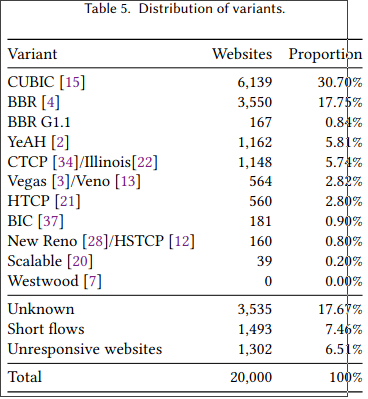
\includegraphics[height=0.9\textheight]{../congest/mishra-et-al-table5}
\imagecredit{Mishra et al, ``The Great Internet TCP Congestion Control Census''}
\end{frame}

\begin{frame}
\frametitle{2023ish measurement data}
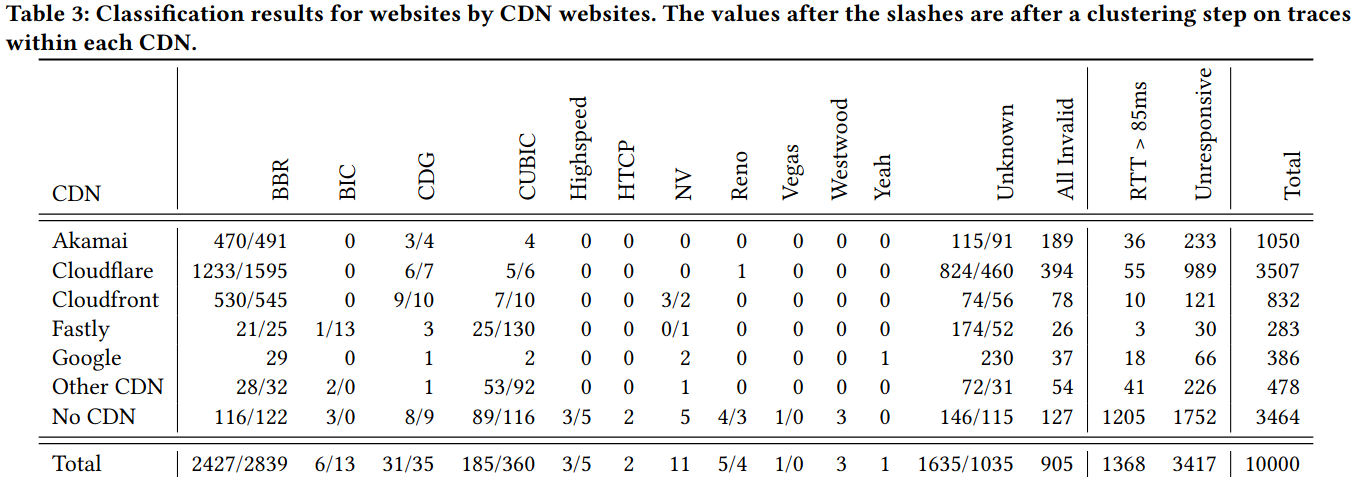
\includegraphics[width=\textwidth]{../congest/ware-et-al-table3}
\imagecredit{Ware et al, ``CCAnalyzer: An Efficient and Nearly Passive Congestion Control Classifier'}
\end{frame}

\begin{frame}
\frametitle{obtaining these measurements}
\begin{itemize}
\item Ware et al (2024) technique: estimate queue occupancy
    \begin{itemize}
    \item add artificial slow link on measurement path
    \item measure number of packets queued over time
    \item shape of graph indicates which congestion control algorithm
    \end{itemize}
\end{itemize}
    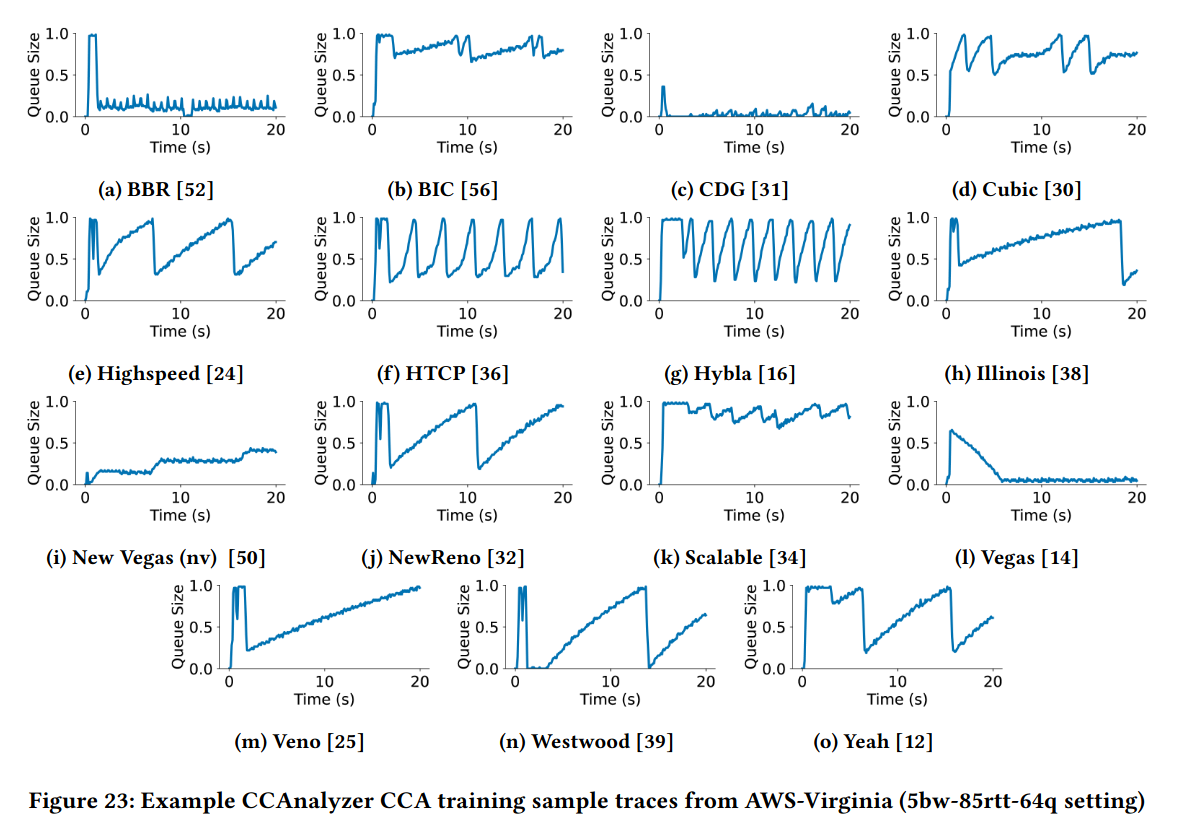
\includegraphics[height=0.5\textheight]{../congest/ware-et-al-fig23}
\end{frame}



% FIXME: options for testing new congestion control/routing/etc.

    % spectrum: model <-> simulation <-> implementation

% Model examples
    % TCP bandwidth
        % flow model for sharing
        % oops, this neglects...
    % TCP bandwidth models
        % complex: https://dl.acm.org/doi/pdf/10.1145/285243.285291
        % simpler: https://dl.acm.org/doi/pdf/10.1145/263932.264023
            % proportional to loss rate idea
        % early: https://dl.acm.org/doi/pdf/10.1145/122431.122434 [1

        % exercise: effect of SACK?
        % exercise: what things does this neglect:

\section{revisiting AIMD model}

\usetikzlibrary{arrows.meta,calc,shapes}

\begin{frame}{picturing sharing}
\begin{tikzpicture}
\tikzset{
    axis/.style={
        draw,ultra thick,-Latex
    },
    normal mark/.style={
        fill=black,
        alt=<5->{fill=black!50},
    },
    normal adjust/.style={
        line width=.5mm,draw=black!50!red,-Latex,
        alt=<5->{draw=black!50!red!50},
    },
}
\begin{scope}[x=1.2cm,y=1.2cm] 
    \path[fill=red!10] (5.5, 0) -- (5.0, 0) -- (0, 5) -- (0, 5.5) -- (5.5, 5.5) -- cycle;
    \path[axis] (0, 0) -- (5.5, 0)
        node[midway,below] {flow 1 bandwidth};
    \path[axis] (0, 0) -- (0, 5.5)
        node[midway,left,align=right] {flow 2\\bandwidth};
    \path[draw,dashed,very thick] (5, 0) -- (0, 5);
    \node[text=red,visible on=<1-3>] at (4, 4) {
        overloaded
    };
    \node[text=black,visible on=<1-3>] at (1.5, 2) {
        underloaded
    };

    \begin{visibleenv}<2>
        \path[draw=black!50,dotted, very thick] (4.5 * 1.2, 2 * 1.2) -- (0, 0);
        \path[line width=1mm,draw=black!50!red,-Latex] (4.5, 2) -- (2.25 * 1.07, 1 * 1.07);
        \path[fill=black] (4.5, 2) circle (2mm);
        \path[fill=black!50] (2.25, 1) circle (2mm);
        \node[anchor=north west,align=left] (incr box) at (4, 4) {
            multiplicative decrease \\
            moves bandwidths along line to origin \\
            example: (90\%, 40\%) to (45\%, 20\%)
        };
        %\draw[violet,very thick] (incr box) -- (4.5, 2+2mm);
    \end{visibleenv}

    \begin{visibleenv}<3>
        \path[draw=black!50,dotted, very thick] (2.25 - 1, 1 - 1) -- (5.5, 1 + 5.5 - 2.25);
        \path[fill=black] (2.25, 1) circle (2mm);
        \path[fill=black!50] (2.25 + 1.3, 1 + 1.3) circle (2mm);
        \node[anchor=north west,align=left] (decr box) at (4, 3) {
            additive decrease \\
            moves bandwidths \\
            at 45-degree angle \\
            example: (45\%, 20\%) to (55\%, 30\%)
        };
    \end{visibleenv}

    \begin{visibleenv}<4->
        \path[normal adjust] (4.5, 2) -- (2.25 * 1.07, 1 * 1.07);
        \path[normal adjust] (2.25 + .14, 1 + .14) -- (2.25 + 1.3 -.14, 1 + 1.3 -.14);
        \path[normal adjust] (2.25 + 1.3 -.14, 1 + 1.3 -.14) -- (1.775*1.07, 1.15*1.07);
        \path[normal adjust] (1.775*1.07, 1.15*1.07) -- (1.775 + 1.3 -.14, 1.15 + 1.3 -.14);
        \path[normal adjust] (1.775 + 1.3 -.14, 1.15 + 1.3 -.14)
            -- (1.5375 * 1.07, 1.225 * 1.07);
        \path[normal adjust] (1.5375 * 1.07, 1.225 * 1.07)
            -- (1.5375 + 1.4 - .14, 1.225 + 1.4 - .14);
        \path[normal adjust] (1.5375 + 1.4 - .14, 1.225 + 1.4 - .14)
            -- (1.4687 * 1.07, 1.325 * 1.07);
        \path[normal mark] (4.5, 2) circle (2mm);
        \path[normal mark] (2.25, 1) circle (2mm);
        \path[normal mark] (2.25 + 1.3, 1 + 1.3) circle (2mm);
        \path[normal mark] (1.775, 1.15) circle (2mm);
        \path[normal mark] (1.775 + 1.3, 1.15 + 1.3) circle (2mm);
        \path[normal mark] (1.5375, 1.225) circle (2mm);
        \path[normal mark] (1.5375 + 1.4, 1.225 + 1.4) circle (2mm);
        \path[normal mark] (1.4687, 1.325) circle (2mm);
    \end{visibleenv}

    \begin{visibleenv}<5->
        \path[draw=black,dashed,very thick] (0,0) -- (5.5, 5.5)
            node[pos=0.75,sloped,above] {equal bandwidth};
    \end{visibleenv}
    \begin{visibleenv}<6>
        \node[anchor=north west,align=left] at (5, 4) {
            multiplicative decrease brings \\
            closer to equal bandwidth line \\
            ~ \\
            additive increase keeps same \\
            distance from line
        };
    \end{visibleenv}
\end{scope}
\end{tikzpicture}
\end{frame}

\begin{frame}{some assumptions we made}
    \begin{itemize}
    \item \ldots that are probably not true
    \vspace{.5cm}
    \item both flows experience drops equally when network overloaded
        \begin{itemize}
        \item higher-bandwidth flow more likely to see drops?
        \item depends on how switches manage queues?
        \item depends on how `bursty' hosts are?
        \end{itemize}
    \item same additive increase factor (for 45 degree angle)
        \begin{itemize}
        \item TCP so far: +1 segment/round-trip-time
        \item round trip time, segment size may vary between flows
        \end{itemize}
    \end{itemize}
\end{frame}


\section{numerical models}

\usetikzlibrary{arrows.meta}
\begin{frame}{models that give numbers?}
    \begin{itemize}
    \item deciding on congestion control 
    \item would like to do math to say how well they'll do
    \vspace{.5cm}
    \item common approach: but gets complicated
    \item simple example: estimating average rate of TCP-like AIMD with no congestion
    \end{itemize}
\end{frame}

\begin{frame}[fragile]{models that give numbers? (1)}
    \begin{itemize}
        \item {\scriptsize figure adapted from Mathis et al, ``The Macroscopic Behavior of the TCP Congestion Avoidance Algorithm''}
    \end{itemize}
\pdftooltip{%
\begin{tikzpicture}
    \draw[very thick,-Latex] (0, 0) -- (0, 4) node[align=center,font=\small,midway,left=0.5cm]{window size\\(packets)}
        node[pos=1.0,left]{W} node[pos=0,left]{0};
    \draw[very thick,-Latex] (0, 0) -- (6, 0) node[font=\small,midway,below=0.5cm] {time (round-trips)};
    \draw[blue, dotted] (0, 2) -- (2, 4);
    \draw[blue] (2, 2) -- (4, 4) -- (4, 2) -- (6, 4);
    \node[anchor=north] at (2, 0) {W/2};
    \node[anchor=north] at (4, 0) {2W/2};
    \node[anchor=north] at (6, 0) {3W/2};
    \begin{visibleenv}<2->
    \path[fill=violet] (0, 0) -- (0, 2) -- (2, 4) -- (2, 0);
    \node[violet,anchor=west,align=left] at (2, 1) {%
        $\frac{W}{2}\cdot \frac{1}{2}\left(\frac{W}{2} + W\right)$ packets sent \\ in one cycle
    };
    \end{visibleenv}
\end{tikzpicture}
}{Graph of window size (in packets) in terms of round trip time, showing a sawtooth pattern, where the window size increases
    from W/2 to W over W round-trips, then decreases to W/2 and repeats the cycle indefinitely.
  The area under the first cycle of the curve is highlighted and calculated to be 
    W/2 times 0.5 times (W/2 + W) [using the area of a trapazoid formula], and is labeled as equal to the number of packets transmitted during the first cycle.}
\end{frame}

\begin{frame}{models that give numbers? (2)}
    \begin{itemize}
    \item $\frac{W}{2}\cdot \frac{1}{2}\left(\frac{W}{2} + W\right)$ per $W/2$ round trips
        \begin{itemize}
        \item $\frac{3W}{4}$ packets per round trip time
        \end{itemize}
    \item packet loss should occur when window size = bandwidth-delay product
        \begin{itemize}
        \item at the capacity of the link(s)
        \end{itemize}
    \item so $W=\text{link BW} \cdot \text{RTT}$
    \item $\implies$ 3/4 link BW achieved total
    \end{itemize}
\end{frame}


\begin{frame}{exercise: what things did this model miss?}
\end{frame}

\begin{frame}{some answers}
    \begin{itemize}
    \item RTT/delay depends on how many packets queued
    \item packet loss could occur for other reasons
        \begin{itemize}
        \item competing connections
        \item network errors
        \end{itemize}
    \item `bursty' connection could trigger packet loss earlier
    \item extra packets being sent for retransmissions
    \item packet loss could trigger timeout/multiple decreases
    \item behavior of other connections sharing links
    \item delays in sending ACKs depending how fast receiver's CPU is
    \item \ldots
    \end{itemize}
\end{frame}

\begin{frame}{more sophisticated models?}
    \begin{itemize}
    \item we can add to formulas to account for other things
    \item this is something people do, but\ldots
    \vspace{.5cm}
    \item most common technique is \textit{discrete event simulation}
    \end{itemize}
\end{frame}

\begin{frame}{interlude: loss rate → transfer rate}
    \begin{itemize}
        \item {\scriptsize adapted from Mathis et al, ``The Macroscopic Behavior of the TCP Congestion Avoidance Algorithm''}
    \item packet loss rate $p$ = 1 per (number of packets sent in W/2 round trips)
    \item $3/4 \times W \times W/2$ packets sent in W/2 round trips
        \begin{itemize}
        \item $p=\frac{3}{8}W^2$
        \end{itemize}
    \item solving for $W = \sqrt{\frac{8}{3p}}$
    \item average transfer rate = $\frac{3}{4}W=C \cdot \sqrt{1/p}$ (for some $C$)
    \end{itemize}
\end{frame}


\section{discrete event simulation}
\usetikzlibrary{arrows.meta}
\begin{frame}{discrete-event simulation}
\pdftooltip{
\begin{tikzpicture}
    % FIXME: queue --> event processing --> more things in queue
    % FIXME: show simulated clock
    % FIXME: show output list of events
    \node[draw,very thick] (queue) {event queue (sorted by time)};
    \node[draw,very thick,anchor=west,dotted] (next ev) at ([xshift=1cm]queue.east) {%
        (time, action)
    };
    \draw[very thick,-Latex] (queue) -- (next ev);
    \node[anchor=north] (run) at ([yshift=-1cm]next ev.south) {run action}; 
    \draw[very thick,-Latex] (next ev) -- (run);
    \node[anchor=west,draw, ultra thick] (network state) at ([xshift=1cm]run.east) {network state};
    \draw[very thick,Latex-Latex] (run) -- (network state);
    \node[draw,dotted] (new events) at (run.west -| queue.south) {new events};
    \draw[very thick,-Latex] (run.west) -- (new events);
    \draw[very thick,-Latex](new events) -- (queue.south);
    \draw[very thick,-Latex] (run.south) -- ++(0cm, -1cm) node[below] (outputs) {outputs};
    \node[anchor=north,font=\small] at (outputs.south) {(example: packet trace, counters)};
    % FIXME: second frame showing example event
\end{tikzpicture}
}{%
    Queue of events sorted by time and the latest event being pulled from the queue. The event pulled out of the queue
    is represented by a tuple of a time and an action. Running the action uses and updates a network state.
    Running the action yields new events, which are added back to the event queue, and outputs like packet traces
    and counters.
}
\end{frame}

\begin{frame}{action example 1}
\begin{itemize}
    \item take next packet from send queue for link X
    \item compute whether packet is lost due to error
    \item compute when packet is done transmitting
        \begin{itemize}
        \item schedule new event to handle next packet in queue at that time
    \end{itemize}
    \item compute reception time of packet on other end of link
        \begin{itemize}
        \item schedule new event to handle packet being received at that time
        \end{itemize}
\end{itemize}
\end{frame}

\begin{frame}{action example 2}
\begin{itemize}
    \item take next packet on link 0 of switch
    \item compute next link for packet
    \item add packet to queue for next link
    \item schedule new events:
        \begin{itemize}
        \item to dequeue from next link (if not scheduled already)
        \end{itemize}
\end{itemize}
\end{frame}


\section{example of NS-3}
\begin{frame}\frametitle{NS-3}
    \begin{itemize}
    \item discrete event simulator planned for AIMD assignment
    \item written in C++
        \begin{itemize}
        \item (yes, I know it's not the most familiar language)
        \item (obvious alternative simulators aren't in better languages\ldots)
        \end{itemize}
    \item create simulations by writing C++ programs
    \end{itemize}
\end{frame}

\begin{FragileFrame}
\frametitle{an NS-3 event handler}
\providecommand{\myemphA}[1]{\myemph<2>{#1}}
\providecommand{\myemphB}[1]{\myemph<3>{#1}}
\providecommand{\myemphC}[1]{\myemph<4>{#1}}
\begin{Verbatim}[fontsize=\fontsize{9}{10},commandchars=\\QX]
bool \myemphAQPointToPointChannel::TransmitStartX(
    Ptr<const Packet> p,
    Ptr<PointToPointNetDevice> src,
    Time txTime
) {
  // ...
  uint32_t wire = src == \myemphBQm_Xlink[0].\myemphBQm_Xsrc ? 0 : 1;

  \myemphCQ\myemphAQSimulator::ScheduleWithContextXX(
    \myemphBQm_Xlink[wire].m_dst->GetNode()->GetId(),
    txTime + \myemphBQm_Xdelay,
    &\myemphAQPointToPointNetDevice::ReceiveX, \myemphBQm_Xlink[wire].m_dst, p->Copy());

  // Call the tx anim callback on the net device
  \myemphBQm_XtxrxPointToPoint(p, src, ...)
  return true;
}
\end{Verbatim}
\begin{tikzpicture}[overlay,remember picture]
    \coordinate (place) at ([yshift=-1cm,xshift=-1cm]current page.north east);
    \tikzset{%
        box/.style={at=(place),anchor=north east,draw=orange!70!black,very thick,align=left,fill=white,font=\small}
    }
    \begin{visibleenv}<2>
        \node[box] {X::Y = Y method/variable of X class};
    \end{visibleenv}
    \begin{visibleenv}<3>
        \node[box] {%
            convention: member variables with \texttt{m\textunderscore} \\
            (C++ member variable $\sim$ Java instance variable)
        };
    \end{visibleenv}
    \begin{visibleenv}<4>
        \node[box] {%
            setup future event; args: \\
            context (for logging mostly) \\
            time event will trigger \\
            method to run + arguments to pass
        };
    \end{visibleenv}
\end{tikzpicture}
\end{FragileFrame}

\begin{FragileFrame}
\frametitle{sample NS-3 simulation --- setup (1)}
{\scriptsize \texttt{ns3/examples/tcp/tcp-bulk-send.cc}}
\begin{Verbatim}[fontsize=\fontsize{9}{10}]
// nodes = routers or endpoints
NodeContainer nodes;
nodes.Create(2);

// create simulated point-to-point link
    // also supported: multi-access links
PointToPointHelper pointToPoint;
pointToPoint.SetDeviceAttribute("DataRate", StringValue("500Kbps"));
pointToPoint.SetChannelAttribute("Delay", StringValue("5ms"));

// setup emulated NICs (which have queues, etc.)
NetDeviceContainer devices;
devices = pointToPoint.Install(nodes);

// setup emulated TCP/IP implementation
InternetStackHelper internet;
internet.Install(nodes);

...
\end{Verbatim}
\end{FragileFrame}

\begin{FragileFrame}
\frametitle{sample  NS-3 simulation --- setup (2)}
{\scriptsize \texttt{ns3/examples/tcp/tcp-bulk-send.cc}}
\begin{Verbatim}[fontsize=\fontsize{9}{10}]
// Simulated "applications" that send/receive data
BulkSendHelper source("ns3::TcpSocketFactory", InetSocketAddress(i.GetAddress(1), port));
source.SetAttribute("MaxBytes", UintegerValue(10000000));
ApplicationContainer sourceApps = source.Install(nodes.Get(0));
sourceApps.Start(Seconds(0));
sourceApps.Stop(Seconds(10));
PacketSinkHelper sink("ns3::TcpSocketFactory", InetSocketAddress(Ipv4Address::GetAny(), port));
ApplicationContainer sinkApps = sink.Install(nodes.Get(1));
sinkApps.Start(Seconds(0));
sinkApps.Stop(Seconds(10));
\end{Verbatim}
\end{FragileFrame}

\begin{FragileFrame}
\frametitle{sample NS-3 simulation --- setup (3)}
{\scriptsize \texttt{ns3/examples/tcp/tcp-bulk-send.cc}}
\begin{Verbatim}[fontsize=\fontsize{9}{10}]
AsciiTraceHelper ascii;

// produces text trace file of simulator events
pointToPoint.EnableAsciiAll(ascii.CreateFileStream("tcp-bulk-send.tr"));

// produces PCAP files you can open in Wireshark
pointToPoint.EnablePcapAll("tcp-bulk-send", false);
\end{Verbatim}
\end{FragileFrame}

% FIXME: show screenshot of wireshark on output
% FIXME: show .tr file



\section{NS-3's TCP modeling and the assignment}
\begin{frame}\frametitle{TCPSocketState}
\begin{itemize}
\item class to track socket state
    \begin{itemize}
    \item regarldess of congestion control algorithm
    \end{itemize}
\item includes (notably for us)
    \begin{itemize}
    \item `congesiton state'
    \item congestion window (cwnd)
    \item slow start threshold (ssthresh)
    \end{itemize}
\end{itemize}
\end{frame}

\begin{frame}\frametitle{TCP congestion states}
\begin{itemize}
\item OPEN --- normal
\item DISORDER --- dupacks/SACKs below threshold for recovery
\item RECOVERY --- retransmitting due to dup-ACK/simple SACK
    \begin{itemize}
    \item temporarily inflated window to account for dropped packets
    \end{itemize}
\item LOSS --- retransmitting due to timeout/etc.
\end{itemize}
\end{frame}

\begin{frame}\frametitle{configurable TCP behavior}
\begin{itemize}
\item TCPRecoveryOps: handle recovery
    \begin{itemize}
    \item EnterRecovery (called on start of retransmitting)
    \item default: cwnd $\rightarrow$ ssthresh
    \item DoRecovery (called for ACK when retransmitting)
    \item default: cwnd $\rightarrow$ cwnd + 1 packet
    \item ExitRecovery (called when `back to normal')
    \item default: cwnd $\rightarrow$ ssthresh
    \end{itemize}
\item \myemph{TCPCongestionOps}:
    \begin{itemize}
    \item IncreaseWindow (called when new segments ACKed)
    \item GetSsThresh (called after loss)
    \end{itemize}
\end{itemize}
\end{frame}


\begin{frame}\frametitle{assingment TCP changes}
\begin{itemize}
\item will customize a \texttt{MyTcpCongestionOps}
\item \ldots which inherits from TCPNewReno
\vspace{.5cm}
\item you can customize increase (IncreaseWindow) and decrease (GetSsThresh)
\end{itemize}
\end{frame}

\begin{FragileFrame}
\frametitle{IncreaseWindow}
\begin{Verbatim}[fontsize=\fontsize{9}{10}]
void
TcpNewReno::IncreaseWindow(Ptr<TcpSocketState> tcb, uint32_t segmentsAcked)
{
    NS_LOG_FUNCTION(this << tcb << segmentsAcked);
 
    if (tcb->m_cWnd < tcb->m_ssThresh)
    {
        segmentsAcked = SlowStart(tcb, segmentsAcked);
    }
 
    if (tcb->m_cWnd >= tcb->m_ssThresh)
    {
        CongestionAvoidance(tcb, segmentsAcked);
    }
}
\end{Verbatim}
\end{FragileFrame}

\begin{FragileFrame}
\frametitle{CongestionAvoidance}
\begin{Verbatim}[fontsize=\fontsize{9}{10}]
void
TcpNewReno::CongestionAvoidance(Ptr<TcpSocketState> tcb, uint32_t segmentsAcked)
{
    NS_LOG_FUNCTION(this << tcb << segmentsAcked);
 
    if (segmentsAcked > 0)
    {
        double adder =
            static_cast<double>(tcb->m_segmentSize * tcb->m_segmentSize) / tcb->m_cWnd.Get();
        adder = std::max(1.0, adder);
        tcb->m_cWnd += static_cast<uint32_t>(adder);
        ...
    }
}
\end{Verbatim}
\begin{itemize}
\item additive increase (plus 1 segment per cwnd)
\end{itemize}
\end{FragileFrame}

\begin{FragileFrame}
\frametitle{SlowStart}
\begin{Verbatim}[fontsize=\fontsize{9}{10}]
uint32_t
TcpNewReno::SlowStart(Ptr<TcpSocketState> tcb, uint32_t segmentsAcked)
{
    NS_LOG_FUNCTION(this << tcb << segmentsAcked);
 
    if (segmentsAcked >= 1)
    {
        tcb->m_cWnd += tcb->m_segmentSize;
        ...
        return segmentsAcked - 1;
    }
 
    return 0;
}
\end{Verbatim}
\begin{itemize}
\item multiplicative increase --- doubling
\end{itemize}
\end{FragileFrame}

\begin{FragileFrame}
\frametitle{GetSsThresh}
\begin{Verbatim}[fontsize=\fontsize{9}{10}]
uint32_t
TcpNewReno::GetSsThresh(Ptr<const TcpSocketState> state, uint32_t bytesInFlight)
{
    NS_LOG_FUNCTION(this << state << bytesInFlight);
 
    return std::max(2 * state->m_segmentSize, bytesInFlight / 2);
}
\end{Verbatim}
\begin{itemize}
\item multiplicative decrease (bytesInFlight / 2)
\end{itemize}
\end{FragileFrame}

\begin{frame}\frametitle{aside: more advanced congestion hooks}
\begin{itemize}
\item TcpCongestionOps also has access to
    \begin{itemize}
    \item ECN (explicit congestion notification) info
    \item timestamps
    \item exactly when duplicate ACKs below threshold/ recovery/etc. occurs
    \end{itemize}
\item used by more advanced TCP implementatoins
\end{itemize}
\end{frame}


\section{aside: NS-3 logging}
\begin{FragileFrame}
\frametitle{NS-3 logging}
    \begin{itemize}
    \item NS3 logging tools
        \begin{itemize}
        \item \url{https://www.nsnam.org/docs/manual/html/logging-asserts.html}
        \end{itemize}
    \item doing logging:
\begin{Verbatim}
// at top of file
NS_LOG_COMPONENT_DEFINE("SomeLabel");
...
// when you want to log
NS_LOG_INFO("value of x=" << x);
    // INFO could be DEBUG, ERROR, ... too
\end{Verbatim}
    \item enabling logging:
        \begin{itemize}
        \item in C++: \texttt{LogComponentEnable("SomeLabel", LOG\_LEVEL\_DEBUG)}
        \item command-line: \texttt{NS\_LOG="SomeLabel=debug" ./ns3 ...}
        \end{itemize}
    \end{itemize}
\end{FragileFrame}



\section{drop-tail and some of its problems}

\usetikzlibrary{arrows.meta,patterns}

\begin{frame}{FIFO + drop-tail}
    \begin{itemize}
    \item \myemph<2-4>{scheduling policy: first-in first-out (FIFO)}
    \item \myemph<5>{drop policy: drop tail}
    \end{itemize}
\begin{tikzpicture}
    \draw[thick] (0, -.5) rectangle (8, .5);
    \begin{visibleenv}<2>
        \path[draw,Latex-,line width=1mm] (0.5, -.5) -- ++(0, -2) node[below] {newest message};
        \path[draw,Latex-,line width=1mm] (7.5, -.5) -- ++(0, -2) node[below] {next out / oldest message};
    \end{visibleenv}
    \begin{visibleenv}<3>
        \path[fill=red!30,pattern=north west lines,pattern color=black] (7, -.5) rectangle ++(1, 1);    
        \path[draw,Latex-,line width=1mm] (7.5, -.5) -- ++(0, -2) node[below] {empty? first message placed here};
    \end{visibleenv}
    \begin{visibleenv}<4>
        \path[fill=violet!30] (5, -.5) rectangle ++(3, 1);    
        \path[fill=red!30,pattern=north west lines,pattern color=black] (4, -.5) rectangle ++(1, 1);    
        \path[draw,Latex-,line width=1mm] (4.5, -.5) -- ++(0, -2) node[below] {partly full? use next slot};
    \end{visibleenv}
    \begin{visibleenv}<5>
        \path[fill=violet!30] (0, -.5) rectangle ++(8, 1);
    \end{visibleenv}
    \foreach \x in {1,2,3,4,5,6,7} {
        \draw (\x, -.5) -- (\x, .5);
    }
    \draw[ultra thick,Latex-] (0, 0) -- ++(-2, 0);
    \draw[alt=<4>{draw=red,text=red},ultra thick,dotted,-Latex] (-.9, 0) to[in=90,out=0] ++(.5,-1) node[below] 
        (discarded text) {discarded};
    \begin{visibleenv}<5>
        \node[anchor=north] at (discarded text.south) {full? discard new packets};
    \end{visibleenv}
    \draw[ultra thick,-Latex] (8, 0) -- ++(2, 0);
    \node[anchor=south] at (.5, .5) {tail};
    \node[anchor=south] at (7.5, .5) {head};
    \begin{visibleenv}<3-5>
        \path[draw,black!50,very thick,dashed,pattern=north west lines, pattern color=black!50]
            (-2.5, -.5) rectangle ++(1, 1);
    \end{visibleenv}
\end{tikzpicture}
\end{frame}




\section{priority queuing}

\usetikzlibrary{arrows.meta,patterns,shapes.misc}

\begin{frame}{priority queue}
    \begin{itemize}
    \item assign priorities to flows
    \item drop packet from lowest priority flow possible
    \item on ties, choose other drop strategy
    \end{itemize}
\end{frame}

\begin{frame}{priority-based dequeue}
\begin{tikzpicture}
\tikzset{
    first flow/.style={pattern=checkerboard,pattern color=blue!30},
    second flow/.style={fill=violet!30},
    ghost/.style={dashed,fill opacity=0.5},
    packet move line/.style={draw,line width=0.8mm},
}
    \begin{scope}[yshift=0cm]
        \foreach \x in {0,1,4,6,7} {
            \path[first flow] (\x, -.5) rectangle ++(1, 1);
        }
        \foreach \x in {2,3,5,8} {
            \path[second flow] (\x, -.5) rectangle ++(1, 1);
        }
        \draw[thick] (0, -.5) rectangle (9, .5);
        \foreach \x in {0,1,2,3,4,5,6,7,8} {
            \draw (\x, -.5) -- (\x, .5);
        }
        \draw[ultra thick] (8, -.5) rectangle ++(1,1);
        \path[packet move line,-{Latex[length=3mm]}] (9, 0) -- ++(1.5, 0);
    \end{scope}

    \begin{scope}[yshift=-2cm]
        \foreach \x in {0,1,3,7,8} {
            \path[first flow] (\x, -.5) rectangle ++(1, 1);
        }
        \foreach \x in {2,4,5,6} {
            \path[second flow] (\x, -.5) rectangle ++(1, 1);
        }
        \draw[thick] (0, -.5) rectangle (9, .5);
        \foreach \x in {0,1,2,3,4,5,6,7,8} {
            \draw (\x, -.5) -- (\x, .5);
        }
        \draw[ultra thick] (6, -.5) rectangle ++(1,1);
        \path[packet move line,-{Latex[length=3mm]}] (6.5, -.5) to[out=-90,in=180] ++(.5, -.5)
            -- ++(2, 0) to[out=0,in=-90] ++(.5, .5) to[in=180,out=90] ++(1, .5);
    \end{scope}
    
    \begin{scope}[yshift=-4cm]
        \foreach \x in {0,1,2,3,4,5,6,7,8} {
            \path[first flow] (\x, -.5) rectangle ++(1, 1);
        }
        \foreach \x in {} {
            \path[second flow] (\x, -.5) rectangle ++(1, 1);
        }
        \draw[thick] (0, -.5) rectangle (9, .5);
        \foreach \x in {0,1,2,3,4,5,6,7,8} {
            \draw (\x, -.5) -- (\x, .5);
        }
        \draw[ultra thick] (8, -.5) rectangle ++(1,1);
        \path[packet move line,-{Latex[length=3mm]}] (9, 0) -- ++(1.5, 0);
    \end{scope}
\end{tikzpicture}
\end{frame}

\begin{frame}{priority-based dropping}
\begin{tikzpicture}
\tikzset{
    first flow/.style={pattern=checkerboard,pattern color=blue!30},
    second flow/.style={fill=violet!30},
    ghost/.style={dashed,fill opacity=0.5},
    packet move line/.style={draw,line width=0.8mm},
}
    \begin{scope}[yshift=-2cm]
        \foreach \x in {0} {
            \draw (\x, -1) rectangle ++(1,1);
            \draw (\x, 0) rectangle ++(1,1);
            \path[first flow,ghost] (\x, -1) rectangle ++(1, 1);
            \node[cross out,draw=red,line width=1mm,minimum width=1cm,minimum height=1cm] at (\x+.5, -.5) {};
            \path[second flow,ghost] (\x, 0) rectangle ++(1, 1);
        }
        \foreach \x in {1,4,6,7,8} {
            \path[first flow] (\x, -.5) rectangle ++(1, 1);
        }
        \foreach \x in {-3,2,3,5} {
            \path[second flow] (\x, -.5) rectangle ++(1, 1);
        }
        \foreach \x in {1,2,3,4,5,6,7,8} {
            \draw (\x, -.5) -- (\x, .5);
        }
        \path[draw] (1, -.5) rectangle (9, .5);
        \path[draw] (-3, -.5) rectangle (-2, .5);
        \path[packet move line,-{Latex[length=3mm]}] (-2, 0) -- (-1.5, 0) to[in=270,out=0]
            (-1., .25) to[in=180,out=90] (-0.75, .5) -- (0, .5);
        \path[packet move line,dotted,-{Latex[length=3mm]}] (.5,-1) -- ++(0, -.5cm);% node[below=-2mm] {discarded};
    \end{scope}
    \begin{scope}[yshift=-4.5cm]
        \foreach \x in {-1.5} {
            \path[first flow,ghost] (\x, -.7) rectangle ++(1, 1);
            \node[cross out,draw=red,line width=1mm,minimum width=1cm,minimum height=1cm] at (\x+.5, -.2) {};
        }
        \foreach \x in {-3,0,1,4,6,7,8} {
            \path[first flow] (\x, -.5) rectangle ++(1, 1);
        }
        \foreach \x in {2,3,5} {
            \path[second flow] (\x, -.5) rectangle ++(1, 1);
        }
        \foreach \x in {1,2,3,4,5,6,7,8} {
            \draw (\x, -.5) -- (\x, .5);
        }
        \path[draw] (0, -.5) rectangle (9, .5);
        \path[draw] (-3, -.5) rectangle (-2, .5);
        \path[packet move line,-{Latex[length=3mm]}] (-2, 0) -- (-2.0, 0) to[in=270,out=0] (-1.75, 0.25) -- (-1.75, .5) to[in=180,out=90] (-1.5, 0.75)
           -- (-1.25, 0.75) to[out=0,in=45+90-45] (-1, .5) -- (-1, -.2+.5);
        \path[packet move line,dotted,-{Latex[length=3mm]}] (-1,-.7) -- ++(0, -.5cm);% node[below=-2mm] {discarded};
    \end{scope}
    \begin{scope}[yshift=-7cm]
        \foreach \x in {-1.5} {
            \path[second flow,ghost] (\x, -.7) rectangle ++(1, 1);
            \node[cross out,draw=red,line width=1mm,minimum width=1cm,minimum height=1cm] at (\x+.5, -.2) {};
        }
        \foreach \x in {-3,0,1,2,3,4,5,6,7,8} {
            \path[second flow] (\x, -.5) rectangle ++(1, 1);
        }
        \foreach \x in {1,2,3,4,5,6,7,8} {
            \draw (\x, -.5) -- (\x, .5);
        }
        \path[draw] (0, -.5) rectangle (9, .5);
        \path[draw] (-3, -.5) rectangle (-2, .5);
        \path[packet move line,-{Latex[length=3mm]}] (-2, 0) -- (-2.0, 0) to[in=270,out=0] (-1.75, 0.25) -- (-1.75, .5) to[in=180,out=90] (-1.5, 0.75)
           -- (-1.25, 0.75) to[out=0,in=45+90-45] (-1, .5) -- (-1, -.2+.5);
        \path[packet move line,dotted,-{Latex[length=3mm]}] (-1,-.7) -- ++(0, -.5cm);% node[below=-2mm] {discarded};
    \end{scope}
\end{tikzpicture}
\end{frame}

\begin{frame}{priority-based dropping (alt)}
\begin{tikzpicture}
\tikzset{
    first flow/.style={pattern=checkerboard,pattern color=blue!30},
    second flow/.style={fill=violet!30},
    ghost/.style={dashed,fill opacity=0.5},
    packet move line/.style={draw,line width=0.8mm},
}
    \begin{scope}[yshift=-2cm]
        \foreach \x in {-1} {
            \path[first flow,ghost] (\x, -.7) rectangle ++(1, 1);
            \node[cross out,draw=red,line width=1mm,minimum width=1cm,minimum height=1cm] at (\x+.5, -.2) {};
        }
        \foreach \x in {0,1,2,3,4} {
            \path[first flow] (\x, -.5) rectangle ++(1, 1);
        }
        \foreach \x in {5.5} {
            \path[second flow,ghost] (\x, -.3) rectangle ++(1, 1);
        }
        \foreach \x in {-4,6.5,7.5} {
            \path[second flow] (\x, -.5) rectangle ++(1, 1);
        }
        \path[draw,thick] (-4, -.5) rectangle (-3, .5);
        \draw[thick] (0, -.5) rectangle (5, .5);
        \draw[thick] (5.5, -.3) rectangle ++(1, 1);
        \draw[thick] (-1, -.7) rectangle ++(1, 1);
        \draw[thick] (6.5, -.5) rectangle (8.5, .5);
        \foreach \x in {0,1,2,3,4,6.5,7.5,8.5} {
            \draw (\x, -.5) -- (\x, .5);
        }
        \path[packet move line,-{Latex[length=3mm]}] (-3, 0) -- (-2.0, 0) to[in=270,out=0] (-1.5, 0.5) to[in=180,out=90] (-.5, 1.2)
           -- (4.5, 1.2) to[out=0,in=45+90-45] (6, 0.7);
        \path[packet move line,dotted,-{Latex[length=3mm]}] (-.5,-.7) -- ++(0, -.5cm);% node[below=-2mm] {discarded};
    \end{scope}
    \begin{scope}[yshift=-4.5cm]
        \foreach \x in {-1.5} {
            \path[first flow,ghost] (\x, -.7) rectangle ++(1, 1);
            \node[cross out,draw=red,line width=1mm,minimum width=1cm,minimum height=1cm] at (\x+.5, -.2) {};
        }
        \foreach \x in {-4,0,1,2,3,4} {
            \path[first flow] (\x, -.5) rectangle ++(1, 1);
        }
        \foreach \x in {5.5,6.5,7.5} {
            \path[second flow] (\x, -.5) rectangle ++(1, 1);
        }
        \path[draw,thick] (-4, -.5) rectangle (-3, .5);
        \draw[thick] (0, -.5) rectangle (5, .5);
        \draw[thick] (5.5, -.5) rectangle ++(1, 1);
        \draw[thick] (-1.5, -.7) rectangle ++(1, 1);
        \draw[thick] (6.5, -.5) rectangle (8.5, .5);
        \foreach \x in {0,1,2,3,4,6.5,7.5,8.5} {
            \draw (\x, -.5) -- (\x, .5);
        }
        \path[packet move line,-{Latex[length=3mm]}] (-3, 0) -- (-3.0, 0) to[in=270,out=0] (-2.5, 0.5) to[in=180,out=90] (-2, 1)
           -- (-1.5, 1) to[out=0,in=45+90-45] (-1, -.2+.5);
        \path[packet move line,dotted,-{Latex[length=3mm]}] (-1,-.7) -- ++(0, -.5cm);% node[below=-2mm] {discarded};
    \end{scope}
    \begin{scope}[yshift=-7cm]
        \foreach \x in {-1.5} {
            \path[second flow,ghost] (\x, -.7) rectangle ++(1, 1);
            \node[cross out,draw=red,line width=1mm,minimum width=1cm,minimum height=1cm] at (\x+.5, -.2) {};
        }
        \foreach \x in {-4,0,1,2,3,4} {
            \path[second flow] (\x, -.5) rectangle ++(1, 1);
        }
        \foreach \x in {5,6,7} {
            \path[second flow] (\x, -.5) rectangle ++(1, 1);
        }
        \path[draw,thick] (-4, -.5) rectangle (-3, .5);
        \draw[thick] (0, -.5) rectangle (5, .5);
        \draw[thick] (5, -.5) rectangle ++(1, 1);
        \draw[thick] (-1.5, -.7) rectangle ++(1, 1);
        \draw[thick] (6, -.5) rectangle (8, .5);
        \foreach \x in {0,1,2,3,4,6,7,8} {
            \draw (\x, -.5) -- (\x, .5);
        }
        \path[packet move line,-{Latex[length=3mm]}] (-3, 0) -- (-3.0, 0) to[in=270,out=0] (-2.5, 0.5) to[in=180,out=90] (-2, 1)
           -- (-1.5, 1) to[out=0,in=45+90-45] (-1, -.2+.5);
        \path[packet move line,dotted,-{Latex[length=3mm]}] (-1,-.7) -- ++(0, -.5cm); % node[below=-2mm] {discarded};
    \end{scope}
\end{tikzpicture}
\end{frame}

\begin{frame}{priority: all or nothing}
    \begin{itemize}
    \item if flow A has greater priority than flow B
    \item and both can use full available bandwidth
    \vspace{.5cm}
    \item flow A gets full available bandwidth
    \item flow B gets no bandwidth (everything dropped)
    \end{itemize}
\end{frame}



\section{simple fair queuing}
% FIXME:
    % with packet arrivals synchornized to packet ends
    % what if arrives-in-middle
    % simultaing bit-by-bit sending

\section{weighted fair queuing}
\begin{frame}{weights instead of priorities}
    \begin{itemize}
    \item alternate idea: weights
    \item if flow A has weight 9, flow B has weight 1
    \item and both can use full availabile bandwidth
    \vspace{.5cm}
    \item flow A gets 90\% of bandwidth
    \item flow B gets 10\% of bandwidth
    \end{itemize}
\end{frame}




\section{backup slides}
\begin{frame}\frametitle{backup slides}
\end{frame}
\section{deep queues?}
\usetikzlibrary{arrows.meta}
\begin{frame}{filling buffers}
\begin{tikzpicture}
\tikzset{
    axis/.style={
        draw,ultra thick,-Latex
    },
    normal mark/.style={
        fill=black,
        alt=<5->{fill=black!50},
    },
    normal adjust/.style={
        line width=.5mm,draw=black!50!red,-Latex,
        alt=<5->{draw=black!50!red!50},
    },
}
\begin{scope}[x=1.2cm,y=1.2cm] 
    \path[fill=red!10] (5.5, 0) -- (5.0, 0) -- (0, 5) -- (0, 5.5) -- (5.5, 5.5) -- cycle;
    \path[axis] (0, 0) -- (5.5, 0)
        node[midway,below] {flow 1 bandwidth};
    \path[axis] (0, 0) -- (0, 5.5)
        node[midway,left,align=right] {flow 2\\bandwidth};
    \path[draw,dashed,very thick] (5, 0) -- (0, 5);
    \node[text=red] at (4, 4) {
        overloaded
    };
    \node[text=black,rotate=-45] at (2.25, 2.25) {
        buffers almost full
    };
    \path[draw,dotted,very thick] (4, 0) -- (0, 4);
\end{scope}
\end{tikzpicture}
\end{frame}

\begin{frame}{big buffers? (in 2011 or so)}
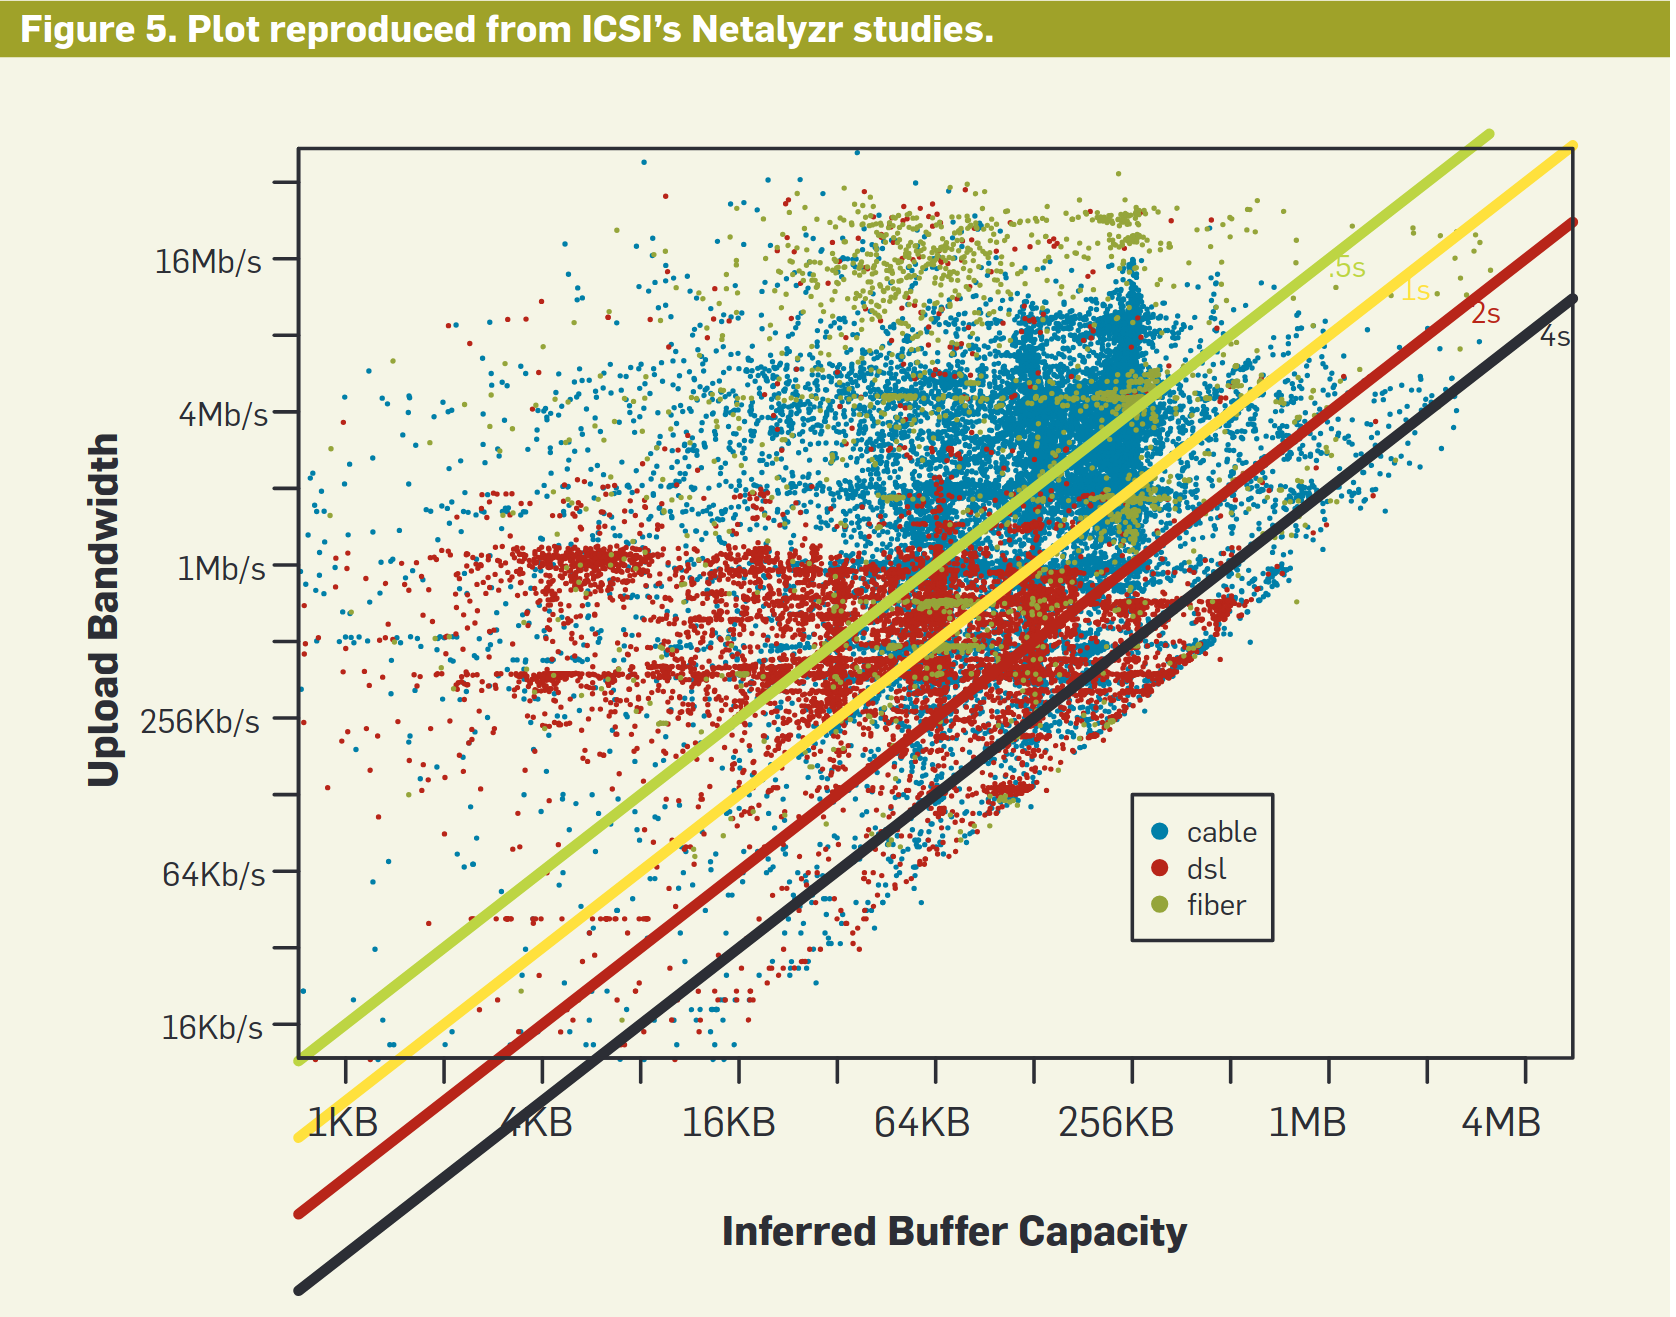
\includegraphics[width=0.6\textwidth]{../congest/cacm-bufferbloat-fig5}

{\scriptsize Jim Gettys and Kathleen Nichols, \\ ``Bufferbloat: Dark Buffers in the Internet'' (CACM, Jan 2012)}
\end{frame}

\begin{frame}{problems with big buffers}
    \begin{itemize}
    \item high latency --- bad for some applications
    \item slower response to congestion
        \begin{itemize}
        \item 1 second round trip time = 1 second to detect congestion
        \item more likely to have `congestion collapse'
        \end{itemize}
    \end{itemize}
\end{frame}

\begin{frame}{avoiding big buffers}
    \begin{itemize}
    \item multiple fixes (that can be combined):
    \vspace{.5cm}
    \item use smaller buffers?
        \begin{itemize}
        \item simpliest solution
        \end{itemize}
    \item detect congestion without full buffer\ldots
        \begin{itemize}
        \item \myemph<3>{by choosing when/which packets to drop better?}
        \item \myemph<4>{by using something other than drops?}
        \end{itemize}
    \end{itemize}
\end{frame}


\subsection{self-clocking and fast retransmit}
\begin{frame}{self-clocking and dup-ACKs}
    \begin{itemize}
    \item without losses, sender sends one new packet per ACK
    \item keeps number of packets in network constant
    \item but duplicate ACKs are exception (say window size 6):
    \end{itemize}
{\fontsize{10}{11}\selectfont
\begin{tabular}{llll}
recv'd & sent & count of packets in flight \\ \hline
--- & data 0-5 & 6 \\
ACK 0 & ~ & 5 \\
~ & data 6 & 6 \\
ACK 1 & ~ & 5 \\
~ & data 7 & 6 \\
ACK 1 & ~  & 5 \\
ACK 1 & ~  & 4 \\
ACK 1 & ~ & 3 \\
~ & data 2 & 4 \\
ACK 1 & ~ & 3 \\
\end{tabular}
}
\end{frame}

\begin{frame}{alternate explanation}
    \begin{itemize}
    \item sender stopped sending while receiving duplicate ACKs
    \item but we know \textit{most messages got there}
    \item means our usage of network doesn't reflect out window size
    \end{itemize}
\end{frame}

\begin{frame}{TCP's fast retransmission}
\begin{itemize}
\item on third duplicate ACK:
\vspace{.5cm}
\item resend packet,
\item do multiplicative decrease, AND THEN
\item temporarily add 2 packet to window for each dup ACK
    \begin{itemize}
    \item send packets to replace received packet
    \item (if allowed by multiplicative-decreased window)
    \end{itemize}
\item reset window size back when later ACK
\end{itemize}
\end{frame}

\begin{frame}{self-clocking and fast retransmit}
\begin{itemize}
\item adjust window size to keep packets in flight constant:
\end{itemize}
{\fontsize{9}{10}\selectfont
\begin{tabular}{llll}
recv'd & sent & count packets in flight & send window size (range) \\ \hline
--- & data 0-5 & 6 & 6 (0-5)\\
ACK 0 & ~ & 5 & 6 (1-6) \\
~ & data 6 & 6 & 6 (1-6)\\
ACK 1 & ~ & 5 & 6 (2-7)\\
~ & data 7 & 6 & 6 (2-7)\\
ACK 1 & ~  & 5 & 6 (2-7)\\
ACK 1 & ~  & 4 & 6 (2-7)\\
ACK 1 & ~ & 3 & 6 (2-7) \\
~ & data 2 & 4 & \myemph{8} (2-9)\\
~ & \myemph{data 8} & 5 & 8 (2-9)\\
~ & \myemph{data 9} & 6 & 8 (2-9)\\
ACK 1 & ~ & 5 & \myemph{9} (2-10)  \\
~ 1 & \myemph{data 10} & 5 & \myemph{9} (2-10)  \\
\end{tabular}
}
\end{frame}


\end{document}
